\documentclass[11pt,letterpaper]{article}
\usepackage[lmargin=1in,rmargin=1in,tmargin=1in,bmargin=1in]{geometry}
\usepackage{../style/homework}
\usepackage{../style/commands}
\setbool{quotetype}{false} % True: Side; False: Under
\setbool{hideans}{false} % Student: True; Instructor: False

% -------------------
% Content
% -------------------
\begin{document}

\homework{2: Due 09/13}{Science is simply common sense at its best; that is, rigidly accurate in observation, and merciless to fallacy in logic.}{Thomas Huxley}

% Problem 1
\problem{10} Show that $P \wedge (\neg Q \vee R) \to (P \wedge R) \vee \neg Q$ is a tautology by constructing its truth table. Using words, explain why this expression is a tautology without making reference to its truth table. \pspace

\sol Constructing the truth table, we have\dots \par
	\begin{table}[!ht]
	\centering
	\begin{tabular}{ccc||ccc|cc||c}
	$P$ & $Q$ & $R$ & $\neg Q$ & $\neg Q \vee R$ & $P \wedge (\neg Q \vee R)$ & $P \wedge R$ & $(P \wedge R) \vee \neg Q$ & $P \wedge (\neg Q \vee R) \to (P \wedge R) \vee \neg Q$ \\ \hline
	T & T & T & F & T & T & T & T & T \\
	T & T & F & F & F & F & F & F & T \\
	T & F & T & T & T & T & T & T & T \\
	T & F & F & T & T & T & F & T & T \\
	F & T & T & F & T & F & F & F & T \\
	F & T & F & F & F & F & F & F & T \\
	F & F & T & T & T & F & F & T & T \\
	F & F & F & T & T & F & F & T & T
	\end{tabular}
	\end{table} \par
Because $P \wedge (\neg Q \vee R) \to (P \wedge R) \vee \neg Q$ is true for every input of $P$, $Q$, and $R$, we know that $P \wedge (\neg Q \vee R) \to (P \wedge R) \vee \neg Q$ is a tautology. \pspace

Now let us explain why $P \wedge (\neg Q \vee R) \to (P \wedge R) \vee \neg Q$ is a tautology without making reference to a truth table. We know that $P \wedge (\neg Q \vee R) \to (P \wedge R) \vee \neg Q$ can only be false if $P \wedge (\neg Q \vee R)$ is true but $(P \wedge R) \vee \neg Q$ is false. Assume that $P \wedge (\neg Q \vee R)$ is true. This means that $P$ is true and $\neg Q \vee R$ is true. Because $\neg Q \vee R$ is true, either $\neg Q$ is true or $R$ is true. But then for $P \wedge (\neg Q \vee R)$ to be true, we know that either $P$ and $\neg Q$ is true, or $P$ and $R$ is true. \pspace

If $P$ and $\neg Q$ is true, then we know $\neg Q$ is true. But then $(P \wedge R) \vee \neg Q$ is true because $\neg Q$ is true. But then $P \wedge (\neg Q \vee R) \to (P \wedge R) \vee \neg Q$ is true. Now if $P$ and $R$ is true, we know that both $P$ and $R$ are true. But then $P \wedge R$ is true so that $(P \wedge R) \vee \neg Q$ is true. But then $P \wedge (\neg Q \vee R) \to (P \wedge R) \vee \neg Q$ is true. Now we see that no matter the combination of inputs for $P$, $Q$, and $R$, the proposition $P \wedge (\neg Q \vee R) \to (P \wedge R) \vee \neg Q$ is true. Therefore, this proposition is a tautology. 



\newpage



% Problem 2
\problem{10} Let $n$ be a fixed natural number. Consider the statement, ``If $n$ is even, then $n$ is not prime or $n$ is 2.''
	\begin{enumerate}[(a)]
	\item By defining appropriate propositions, write the given statement as a logical expression.
	\item Write the converse of your answer in (a). Then write this logical expression in words. Is this statement always true? Explain.
	\item Write the contrapositive of your answer in (a). Then write this logical expression in words. Is this statement always true? Explain. 
	\end{enumerate} \pspace

\sol
\begin{enumerate}[(a)]
\item Fix an integer $n$. Let $P$ be the proposition that ``$n$ is even,'' let $Q$ be the proposition that ``$n$ is prime,'' and $R$ be the proposition that ``$n$ is 2.'' Then the statement ``If $n$ is even, then $n$ is not prime or $n$ is 2'' can be written as $P \to \neg Q \vee R$. \pspace

\item The converse of $P \to \neg Q \vee R$ is $\neg Q \vee R \to P$. In words, the proposition $\neg Q \vee R$ is ``if $n$ is not prime or $n$ is 2, then $n$ is even.'' This statement is not always true. As a counterexample, choose $n= 9$. Then $n$ is not prime so that ``$n$ is not prime or $n$ is 2'' is true. But $n$ is not even, so that the statement ``if $n$ is not prime or $n$ is 2, then $n$ is even'' is false. \pspace

\item The contrapositive of $P \to \neg Q \vee R$ is $\neg (\neg Q \vee R) \to \neg P \equiv Q \wedge \neg R \to \neg P$. In words, the proposition $Q \wedge \neg R \to \neg P$ is ``if $n$ is prime and $n$ is not 2, then $n$ is not even.'' The statement is always true. If $n$ is prime, then $n$ is one of $2, 3, 5, 7, \ldots$. If $n$ were an even number greater than 2, then $n$ would be divisible by 2 and hence not prime. So if $n$ is a prime that is not 2, it must be odd. But then $n$ is not even. Therefore, the statement ``if $n$ is prime and $n$ is not 2, then $n$ is not even'' is true. 
\end{enumerate}



\newpage



% Problem 3
\problem{10} Suppose the statement, ``If this metal is glowing red, then its temperature must be at least 460$^\circ$C,'' is true. Indicate whether the following statements are true or false. No justification is necessary.
	\begin{enumerate}[(a)]
	\item If the temperate of the metal is at least 460$^\circ$C, then it is glowing red.
	\item If the temperature of the metal is less than 460$^\circ$C, then it is not glowing red.
	\item The metal will only glow red if its temperature is at least 460$^\circ$C.
	\item If the metal is now glowing red, then its temperature is less than 460$^\circ$C.
	\item A necessary condition for the metal to glow red is that its temperature be at least 460$^\circ$C.
	\item A sufficient condition for the metal to glow red is that its temperature is at least 460$^\circ$C.
	\end{enumerate} \pspace

\sol Suppose that the temperature of the metal is $T$. Let $P$ be the proposition ``the metal is growing red,'' $Q$ be the proposition $T \geq 460^\circ \text{C}$. Then the statement ``If this metal is glowing red, then its temperature must be at least 460$^\circ$C'' can be written as $P \to Q$. Because this statement is true, we know that either $P$ is false, i.e. the metal is not glowing red, or both $P$ and $Q$ are true, i.e. the metal is glowing red and its temperature is at least 460$^\circ$C. 

\begin{enumerate}[(a)]
\item This can be written as $Q \to P$.

\item This can be written as $\neg Q \to \neg P$.

\item This can be written as 

\item This can be written as  

\item This can be written as  

\item This can be written as  
\end{enumerate}



\newpage



% Problem 4
\problem{10} Suppose one defines a logical connective `$\boxplus$' by saying that $P \boxplus Q$ is true if and only if \textit{both} $P$ and $Q$ are true.
	\begin{enumerate}[(a)]
	\item Construct the truth table for $P \boxplus Q$.
	\item Using a truth table, show that $(P \boxplus Q) \equiv (P \leftrightarrow Q) \wedge P$ and $(P \boxplus Q) \equiv (P \leftrightarrow Q) \wedge Q$.
	\item Without referencing a truth table, explain the logical equivalences in (b).
	\item Using the result from (b)---but without referencing a truth table---explain why $\big( (P \boxplus Q) \big) \leftrightarrow \big( (P \leftrightarrow Q) \wedge P \big)$ and $\big( (P \boxplus Q) \big) \leftrightarrow \big( (P \leftrightarrow Q) \wedge P \big)$ are tautologies. 
	\item Without using a truth table, explain why $P \boxplus Q \equiv Q \boxplus P$.
	\end{enumerate} \pspace

\sol 
\begin{enumerate}[(a)]
\item By definition, we know that $P \boxplus Q$ is true only when both $P$ and $Q$ are true. Then we know that the truth table must be\dots \par
	\begin{table}[!ht]
	\centering
	\begin{tabular}{cc|c}
	$P$ & $Q$ & $P \boxplus Q$ \\ \hline
	T & T & T \\
	T & F & F \\
	F & T & F \\
	F & F & F
	\end{tabular}
	\end{table} \par
[Note: This is just the truth table for $P \wedge Q$ so that we must have $P \boxplus Q \equiv P \wedge Q$.] \pspace

\item We can show that these are logically equivalent using a truth table: the truth values of $P \boxplus Q$ and $(P \leftrightarrow Q) \wedge P$ and $P \boxplus Q$ and $(P \leftrightarrow Q) \wedge Q$ match for each input of $P$ and $Q$ \par
	\begin{table}[!ht]
	\centering
	\begin{tabular}{cc||c|c|cc}
	$P$ & $Q$ & $P \boxplus Q$ & $P \leftrightarrow Q$ & $(P \leftrightarrow Q) \wedge P$ & $(P \leftrightarrow Q) \wedge Q$ \\ \hline
	T & T & T & T & T & T \\
	T & F & F & F & F & F \\
	F & T & F & F & F & F \\
	F & F & F & T & F & F
	\end{tabular}
	\end{table}
Therefore, by the truth table above, we have $(P \boxplus Q) \equiv (P \leftrightarrow Q) \wedge P$ and $(P \boxplus Q) \equiv (P \leftrightarrow Q) \wedge Q$. \pspace

\item We know that $P \boxplus Q$ is true if and only if both $P$ and $Q$ are true. We know that $(P \leftrightarrow Q) \wedge P$ is true if and only if both $P \leftrightarrow Q$ is true and $P$ is true. Now $P \leftrightarrow Q$ is true if and only if the truth values for $P$ and $Q$ match. But then $(P \leftrightarrow Q) \wedge P$ is true if and only if the truth values for $P$ and $Q$ match and $P$ is true, i.e. both $P$ and $Q$ are true. But this precisely the criterion for $P \boxplus Q$ to be true. Therefore, $P \boxplus Q \equiv (P \leftrightarrow Q) \wedge R$. The same explanation holds for $P \boxplus Q \equiv (P \leftrightarrow Q) \wedge Q$ by interchanging the roles of $P$ and $Q$, i.e. it holds mutatis mutandis. \pspace

\item 
\item 
\end{enumerate}



\newpage



% Problem 5
\problem{10} Find a Boolean expression that represents the following circuit and construct its input/output table.
	\begin{figure}[!ht]
	\centering
	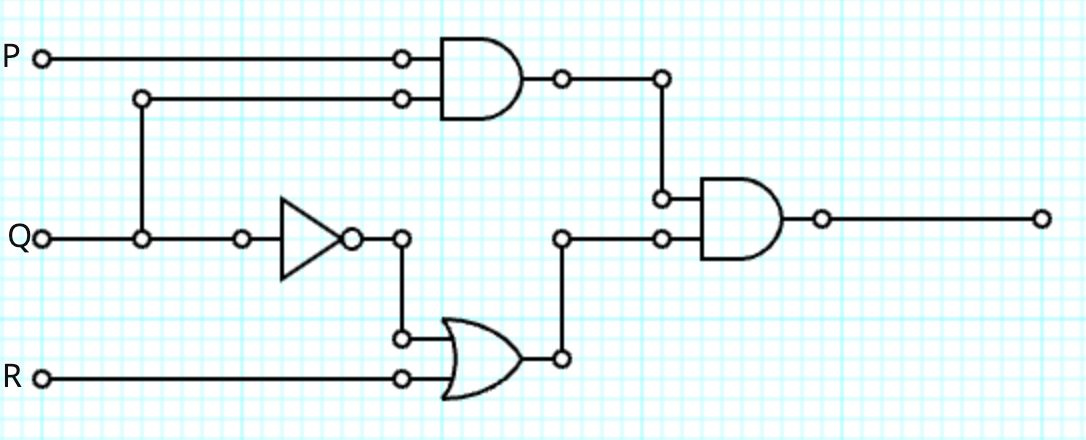
\includegraphics[width=0.75\textwidth]{circuit.png}
	\end{figure} \pspace

\sol 



\newpage



% Problem 6
\problem{10} Draw a circuit diagram corresponding to the Boolean expression $\neg (P \vee Q) \wedge Q$. \pspace

\sol 



\newpage



% Problem 7
\problem{10} Suppose a certain tax exemption applies to individuals that make less than than \$55,000 a year, or have three dependents and have at least \$6,000 in charitable donations. Define appropriate propositions and write the condition for this tax exemption as a Boolean expression. Then construct a circuit diagram corresponding to this Boolean expression. \pspace

\sol 



\newpage



% Problem 8
\problem{10} Watch at least one of the following videos:
	\begin{itemize}
	\item \href{https://www.youtube.com/watch?v=QZwneRb-zqA&ab_channel=SebastianLague}{Exploring How Computers Work}
	\item \href{https://www.youtube.com/watch?v=I0-izyq6q5s&ab_channel=SebastianLague}{How Do Computers Remember?}
	\end{itemize}
Then as thoroughly as possible, comment on what you observed and learned from the video. Be sure to remark as much as possible on how these videos connect to the course content. \pspace

\vfill
\begin{center} {\itshape Solutions will vary.} \end{center}
\vfill


\end{document}